\caption{Construction of the primary longitudinal cohort. Counts are reproduced from the retained aggregate cohort-flow table; the final analytic sample contains students who passed their first real observed MU attempt, subsequently had a numeric Calculus I grade, had CMAT coverage and valid classroom-relative performance measures in both courses, and progressed to Calculus I in the next regular term.}
\label{fig:cohort-flow}
\end{figure}

The 3,389 students who satisfy all conditions except the next-regular-term restriction form a delayed-progression sensitivity cohort in the historical longitudinal analysis. A broader 4,211 future-Calculus progressor cohort is also documented in the methodology record, but it is not yet fully reconciled with the stricter longitudinal pipeline and is therefore not substituted silently for the primary estimand in this draft.

\draftnote{Re-run and report the broad $N=4{,}211$ progressor sensitivity with the same persistence definitions after the longitudinal and methodology pipelines are fully reconciled. The primary paper should state clearly which population each estimate targets.}

\subsection{Exposure and outcomes}

The primary predictor is the number of recorded CMAT visits during the student's MU period, grouped as shown in \Cref{eq:mu-visit-groups}.
\begin{equation}
0,\quad 1\text{--}2,\quad 3,\quad 4+.
\label{eq:mu-visit-groups}
\end{equation}
The exactly-three group corresponds to the operational institutional threshold and the four-or-more group captures recorded use beyond that threshold.

The primary outcome is any recorded CMAT use during the subsequent eligible Calculus I period. This outcome is binary and measures later formal support use, not academic achievement.

The secondary academic outcome is classroom-relative Calculus performance, defined in \Cref{eq:classroom-relative-performance}. For student $i$ in classroom $c$,
\begin{equation}
Z_{ic}=\frac{Y_{ic}-\bar{Y}_{c}}{s_c},
\label{eq:classroom-relative-performance}
\end{equation}
where $c$ is defined by professor, course, and academic period. Classroom reference distributions use numeric grades from eligible real attempts rather than only the final longitudinal subsample.

\subsection{Statistical analysis}

We first estimate the probability of any later CMAT use for each MU visit group and report Wilson 95\% confidence intervals. A Pearson chi-square test summarizes the global association between the four MU groups and later use, with Cram\'er's $V$ as an effect-size measure.

The pre-specified threshold-neighbour comparison contrasts students with exactly three MU visits against students with four or more. We report the risk difference with a Newcombe confidence interval, the risk ratio, odds ratio, Pearson test, and two-sided Fisher exact test. This is an observational risk comparison.

We then estimate logistic regressions for later Calculus use. The adjusted model includes MU visit group, prior classroom-relative MU performance ($Z_{MU}$), official degree programme at the MU attempt, and MU academic period. Standard errors are clustered by MU classroom.

As an exploratory description of the shape of the relationship, a piecewise visit-count model allows one slope through three visits and a second slope after three. The model is descriptive and is not interpreted as regression discontinuity.

For the secondary academic outcome, we estimate linear models of $Z_{Calc}$ including $Z_{MU}$ and MU visit group, followed by a specification that additionally adjusts for official degree programme in Calculus and Calculus period. Standard errors are clustered by Calculus classroom.

\draftnote{Before submission, add a dedicated selection analysis for entry into the longitudinal cohort. Conditioning on passing MU and subsequently reaching Calculus changes the target population and may induce selection. At minimum, compare observed baseline characteristics across retained and excluded progression groups; if defensible pre-exposure covariates become available, consider inverse-probability or related sensitivity analyses.}

\section{Results}

\subsection{Persistence of formal support use}

Later CMAT use differs sharply by prior MU engagement (\Cref{tab:persistence}). Among students with no recorded MU visits, 426 of 2,470 (17.25\%) used CMAT during Calculus. The corresponding proportions were 43.43\% for students with 1--2 MU visits, 54.37\% for exactly three visits, and 66.84\% for four or more.

\begin{table}[htbp]
\centering
\caption{Later CMAT use in Calculus I by prior MU visit group}
\label{tab:persistence}
\begin{tabular}{lrrrr}
\toprule
MU visits & $N$ & Later users & Probability & 95\% CI \\
\midrule
0 & 2,470 & 426 & 17.25\% & [15.81\%, 18.79\%] \\
1--2 & 472 & 205 & 43.43\% & [39.03\%, 47.94\%] \\
3 & 103 & 56 & 54.37\% & [44.77\%, 63.66\%] \\
4+ & 196 & 131 & 66.84\% & [59.98\%, 73.05\%] \\
\bottomrule
\end{tabular}
\end{table}

The global association is strong: $\chi^2(3)=392.47$, $p=9.47\times10^{-85}$, with Cram\'er's $V=.348$. The minimum expected cell count is approximately 26, so sparse expected cells do not drive the Pearson result.

\begin{figure}[htbp]
\centering
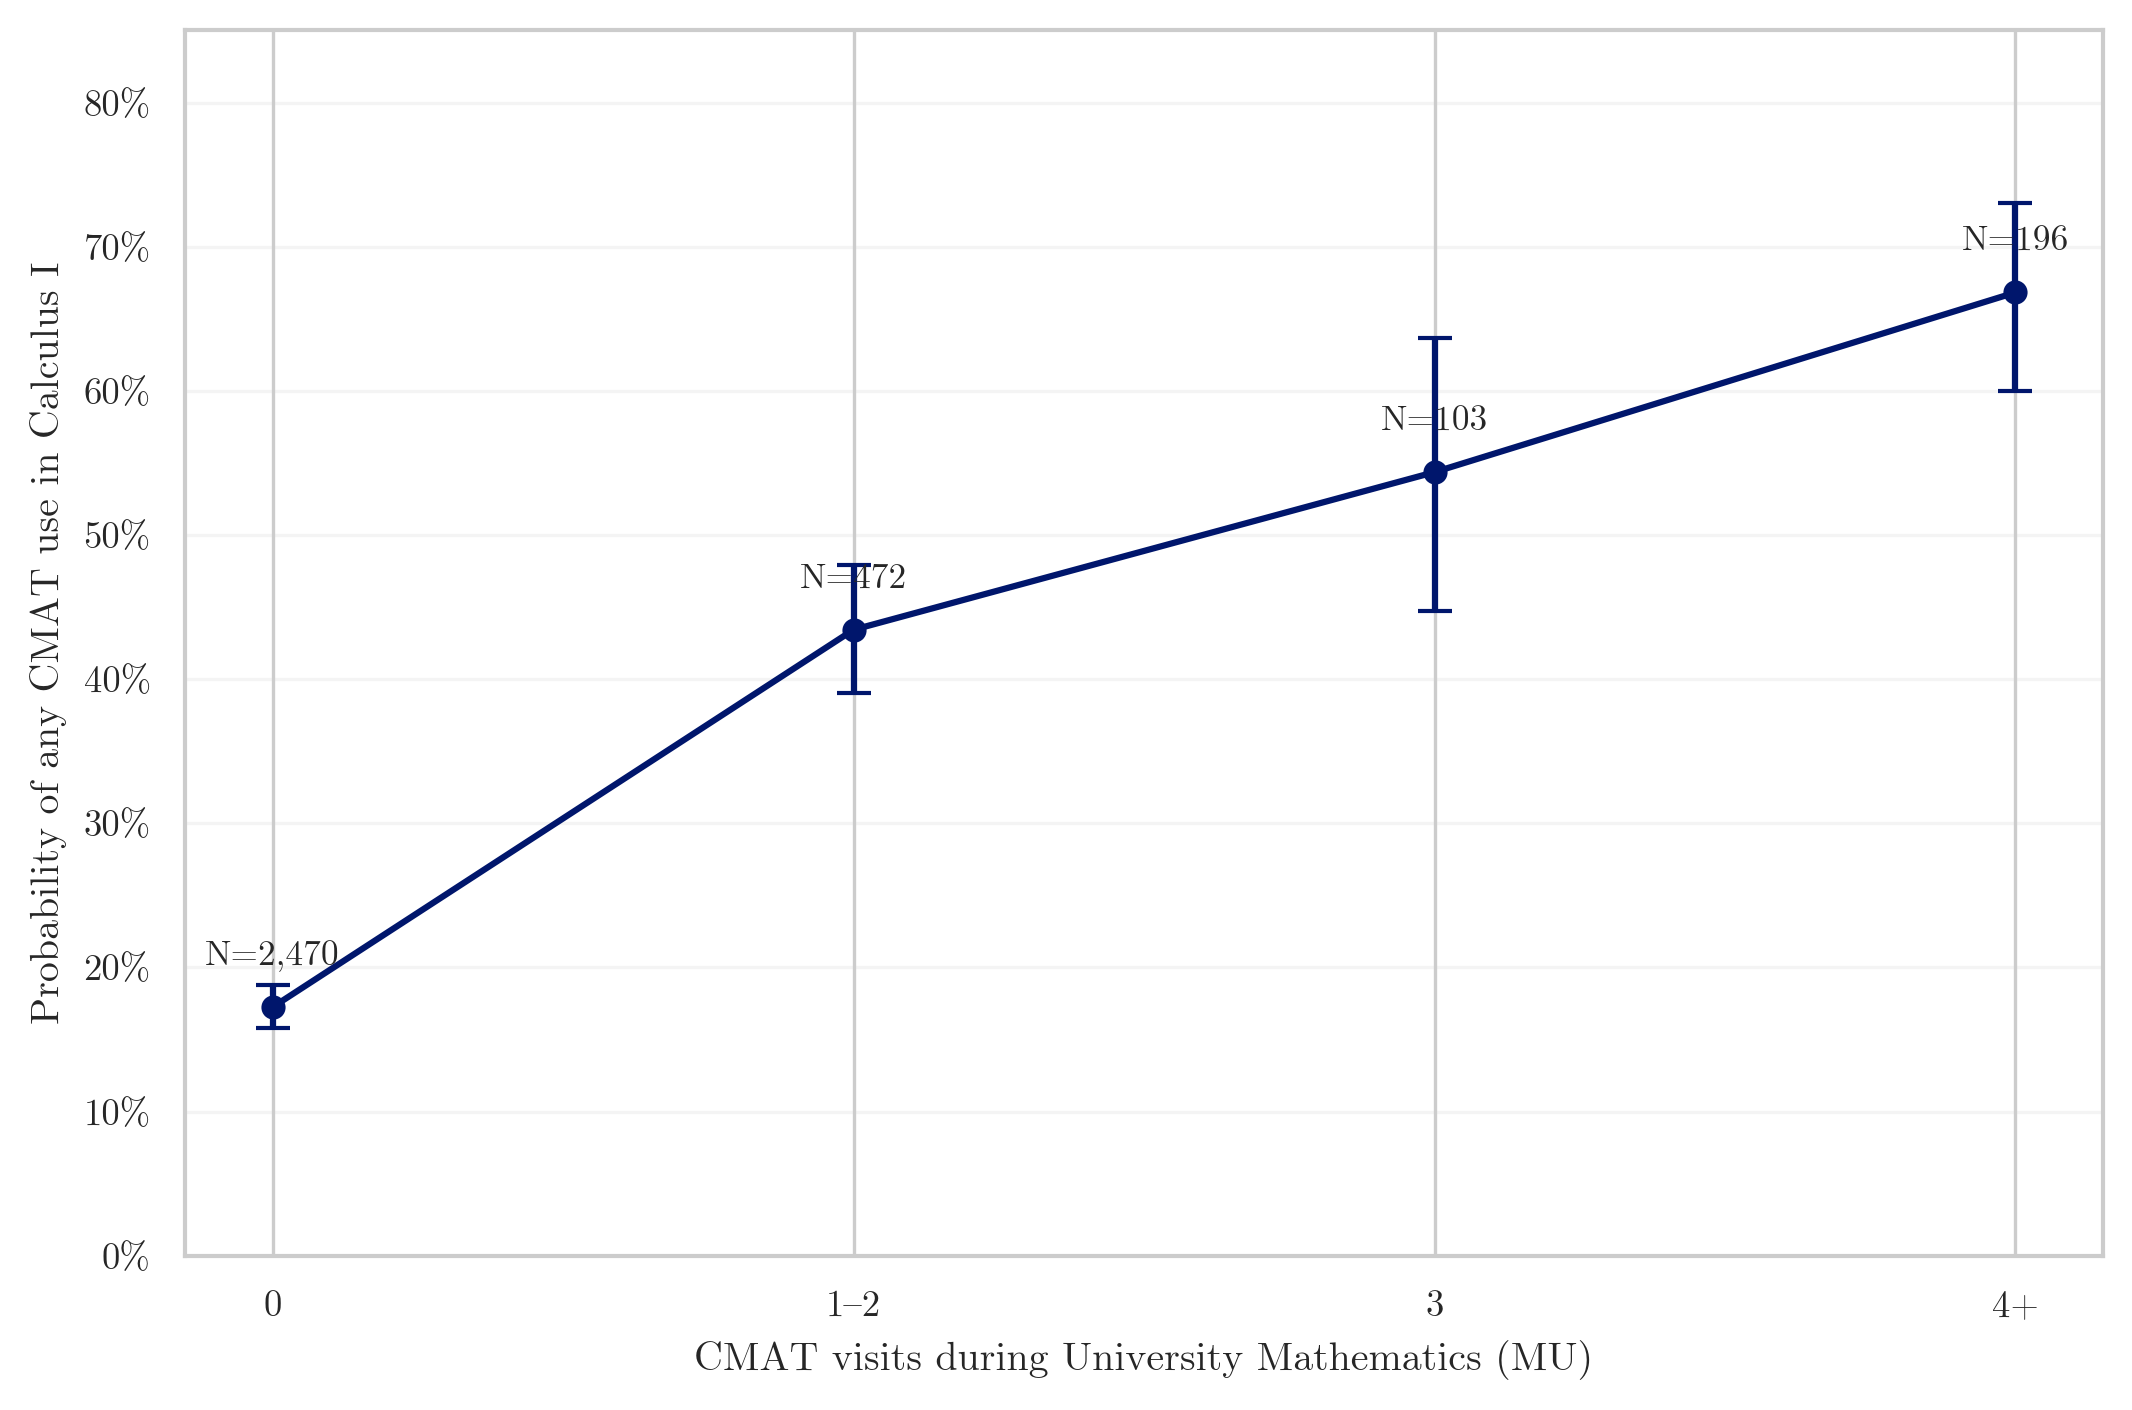
\includegraphics[width=0.78\textwidth]{../results/figures/figure_02_main_persistence.png}
\caption{Probability of any CMAT use during Calculus I by prior University Mathematics (MU) visit group in the primary longitudinal cohort ($N=3{,}241$). Points show observed group proportions and error bars show Wilson 95\% confidence intervals.}
\label{fig:persistence}
\end{figure}

\subsection{Exactly three versus four or more visits}

The comparison most directly tied to the institutional threshold contrasts exactly three visits with four or more. Later CMAT use was 54.37\% in the exactly-three group and 66.84\% in the four-or-more group. The risk difference was 12.47 percentage points (95\% CI [0.92, 23.90]). The risk ratio was 1.229 (95\% CI [1.004, 1.505]) and the odds ratio was 1.691 (95\% CI [1.038, 2.757]). The Pearson test gave $p=.0343$ and Fisher's exact test gave $p=.0440$.

The comparison is consistent with behavioural heterogeneity around the operational threshold: students who continued beyond three MU visits were more likely to use CMAT again later than students who stopped exactly at three. It does not establish that crossing three visits caused persistence, because the number of visits is student-controlled.

\subsection{Visit-count shape around the threshold}

A descriptive piecewise model shows a much steeper association between visit count and later use through three visits than after three. Up to the threshold, the estimated odds ratio per additional visit is 1.994 (95\% CI [1.807, 2.200], $p<.001$). Beyond three visits, the corresponding odds ratio is 1.063 (95\% CI [0.982, 1.150], $p=.131$). \Cref{fig:threshold-piecewise} summarizes this contrast. The flattening is descriptive; it does not identify a discontinuity caused by the institutional threshold.

\begin{figure}[htbp]
\centering
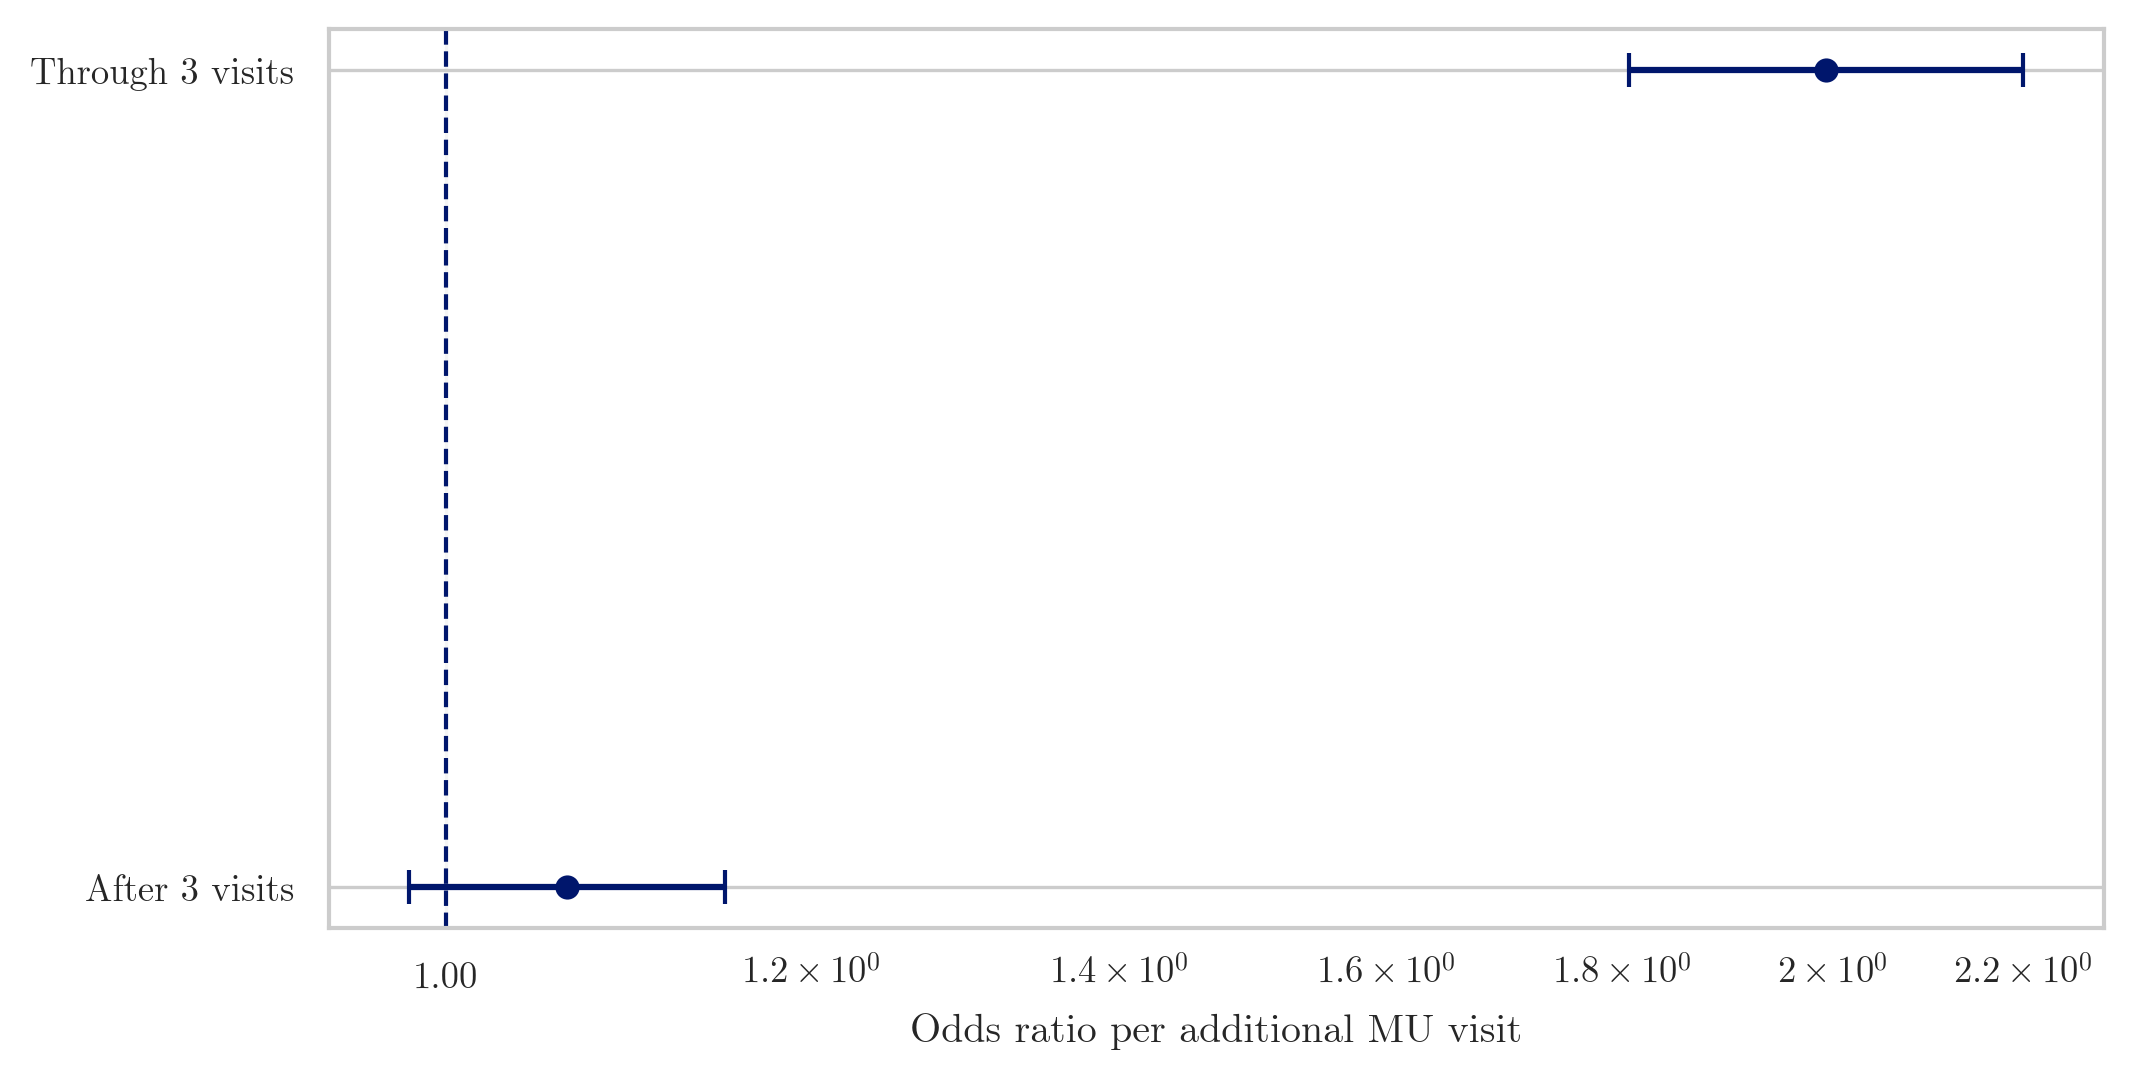
\includegraphics[width=0.72\textwidth]{../results/figures/figure_03_threshold_piecewise.png}
\caption{Estimated per-visit odds ratios from the descriptive piecewise logistic model of later CMAT use, with cluster-robust 95\% confidence intervals. The first slope applies through three MU visits and the second applies after three visits. The dashed reference line denotes an odds ratio of 1. Visit count is student-controlled, so the figure is not a regression-discontinuity estimate.}
